\documentclass{article}
\usepackage[margin=1.5cm,includefoot,footskip=30pt]{geometry}
\usepackage{apacite}
\usepackage{booktabs}
\usepackage{amsmath}
\usepackage{graphicx}
\usepackage{float}

\title{Research Proposal}
\author{Yuheng Wang}
\date{\today}
\begin{document}
\maketitle
\section{Introduction}\label{first_section}

\setlength{\parindent}{0pt}

Research question: Self-selection and inter-provincial migration in China\\

This paper is the first to apply Roy$'$s self-selection model to understand the inter-provincial migration in China. The model predicts that inter-provincial differences in the returns to skills and mean income level are major determinants of both the size and skill composition of inter-provincial migration flows in China. Using data from China Family Panel Studies from 2010 to 2016, this paper also provides an empirical analysis to test for the two predictions from Roy model: correlation between skill levels and out-migration rates should be more positive in provinces with lower returns to skills, and skilled workers should move to states with higher returns to skills.

% Table generated by Excel2LaTeX from sheet 'Sheet1'
\begin{table}[htbp]
  \centering
  \caption{In-Migration Rate, income, and education across provinces in China}
    \begin{tabular}{lrrrr}
              &       &       &       &  \\
    \toprule
    Province & \multicolumn{1}{l}{N} & \multicolumn{1}{l}{Income} & \multicolumn{1}{l}{Education} & \multicolumn{1}{l}{ Rate} \\
    \midrule
          &       &       &       &  \\
    Beijing & 101   & 22410 & 11    & 0.51 \\
    Tianjin & 116   & 23896 & 8.9   & 0.23 \\
    Hebei & 946   & 10412 & 7.6   & 0.042 \\
    Shanxi & 659   & 10958 & 7.8   & 0.029 \\
    Liaoning & 1516  & 12456 & 8.4   & 0.078 \\
    Jilin & 300   & 10297 & 7.8   & 0.13 \\
    Heilongjiang & 533   & 11613 & 8.1   & 0.26 \\
    Shanghai & 1220  & 24733 & 9     & 0.19 \\
    Jiangsu & 351   & 16379 & 7     & 0.1 \\
    Zhejiang & 318   & 20765 & 7.9   & 0.12 \\
    Anhui & 299   & 13191 & 5.8   & 0.033 \\
    Fujian & 206   & 11030 & 5.5   & 0.053 \\
    Jiangxi & 322   & 10387 & 6     & 0.016 \\
    Shandong & 855   & 11180 & 7.1   & 0.042 \\
    Henan & 1950  & 9447  & 7.6   & 0.041 \\
    Hubei & 244   & 16419 & 8.2   & 0.094 \\
    Hunan & 514   & 14583 & 8.6   & 0.056 \\
    Guangdong & 1449  & 12634 & 7.3   & 0.1 \\
    Guangxi & 387   & 7490  & 6.7   & 0.013 \\
    Chongqing & 153   & 7935  & 5.2   & 0.35 \\
    Sichuan & 976   & 8323  & 5.1   & 0.025 \\
    Guizhou & 535   & 7033  & 4.7   & 0.015 \\
    Yunnan & 534   & 9697  & 5.8   & 0.017 \\
    Shaanxi & 423   & 12413 & 7.4   & 0.08 \\
    Gansu & 1835  & 7805  & 5.8   & 0.026 \\
          &       &       &       &  \\
    \midrule
    All province & 1086  & 11999 & 7.2   & 0.075 \\
    \bottomrule
    \end{tabular}%
  \label{table1}%
\end{table}%


\section{Literature review}\label{second_section}

The early empirical study of Chinese migration flows focused on explaining the rural-to-urban migration. Zhao points out that the abundance of household labor and the shortage of farmland are among the most important determinants of labor migration, which can be predicted by Lewis$'$ dual sector model\,\cite{zhao_labor_1999}. However, many studies have shown that wages of hired workers in the agricultural sector have increased dramatically since 2003, and China has reached its Lewis turning point before 2010\,\cite{zhang_china_2011,cai_wage_2011}. Under such circumstances, we can shift our emphasis from rural-urban migration to a more general study of the determinant of Chinese labor migration. Several later papers emphasize the mean income difference as the crucial determinant of labor migration in China\,\cite{zhu_impacts_2002}. These results follow from Hicks-Sjaastad model which predicts that income differentials (minus migration costs) generate unidirectional migration flows\,\cite{sjaastad_costs_1962, hicks_theory_1963}.\\


However, statistics from China Family Panel Studies (will be described in the final section) shown in Table 1 suggest that all provinces have in-migration and many low-income provinces, including Jilin, Heilongjiang, and Chongqing, have more than 10\% residents as in-migrants. This is to say that China has bidirectional migration between provinces. To understand such phenomenon, this paper employs the general Roy model which first proposed by Roy and later applied to migration by Borjas\,\cite{borjas_self-selection_1992}. It stresses regional differences in the returns to skills (as well as regional differences in mean income) and predicts that regions that pay higher returns to skills attract more skilled workers than regions that pay lower returns. Table 2 presents means of the income and education for movers and non-movers. On average, movers are more skilled and have much higher income than non-movers.

% Table generated by Excel2LaTeX from sheet 'Sheet1'
\begin{table}[htbp]
  \centering
  \caption{Means of variable by movers}
    \begin{tabular}{lrrr}
    &       &       &  \\
    \toprule
    & \multicolumn{1}{l}{Overall sample} & \multicolumn{1}{l}{Movers} & \multicolumn{1}{l}{Nonmovers} \\
    \midrule
    Age   & 45.29939 & 44.51994 & 45.24101 \\
    Percent male & 0.5502324 & 0.4968102 & 0.546231 \\
    Income & 11562.37 & 17396.86 & 11999.38 \\
    Years of education & 7.112345 & 8.070175 & 7.184088 \\
    Sample size & 16742 & 1254  & 15488 \\
    \bottomrule
    \end{tabular}%
  \label{table2}%
\end{table}%

\section{The Model}\label{third_section}

This paper$'$s theory is based on Roy self-selection model formalized by Borjas\,\cite{borjas_self-selection_1987}. Assume a country is divided into k distinct regions, indexed by i=1,...,k. Individuals maximize their income by choosing residence in one of the regions. We also assume that initial distribution of individual skills is the same in all regions. The population log earnings distribution in region i is given by

\begin{equation}\label{1_math}
log\,w_{i} = \mu_{i} + v_{i}, \hspace{20pt} i = 1,...,k
\end{equation}

where $\mu_{i}$ is the mean income in region i, and $v_{i}$ is a random variable that measures person-specific deviation from mean income in region i.

An income-maximizing individual chooses to reside in region j whenever

\begin{equation}\label{2_math}
log\,w_{j} > \max_{i\neq j}\,\{log\, w_{i} \}
\end{equation}

A simplifying assumption which allows a complete characterization of the equilibrium sorting is that individual earnings are perfected correlated across regions, that is, $Corr(v_{i},v_{j})=1$ for all i, j. In this case, we can write the population income distribution of region i as

\begin{equation}\label{1a_math}
log\,w_{i} = \mu_{i} + \eta_{i}v, \hspace{20pt} i = 1,...,k \tag{1a}
\end{equation}

Here, $v$ represents individual-specific skills, and the coefficient can be interpreted as the "rate of return" to skills in region i. To simplify the results, it is convenient to label the regions such that they are ranked in terms of $\eta$ with $\eta_{1}<\eta_{2}<...<\eta_{k}$. Using equations (\ref{1a_math}) and (\ref{2_math}) repetitively, we can deduce the following inequalities
%\begin{subequations}
%\begin{align}
%&\text{Choose region 1:\hspace{10pt}} v < \min_{i=2,...,k}\,\left\{\frac{\mu_{1}-\mu_{i}}{\eta_{i}-\eta_{1}}\right\}      \label{3a_math}\\
%&\text{Choose region j:\hspace{10pt}} \max_{i=1,...,j-1}\left\{\frac{\mu_{i}-\mu_{j}}{\eta_{j}-\eta_{i}}\right\} <v<\min_{i=j+1,...,k}\left\{\frac{\mu_{j}-\mu_{i}}{\eta_{i}-\eta_{j}}\right\}   \label{3b_math}  \\
%&\text{Choose region k:\hspace{10pt}} v>\max_{i=1,...,k-1}\left\{\frac{\mu_{i}-\mu_{k}}{\eta_{k}-\eta_{i}}\right\}   \label{3c_math}
%\end{align}
%\end{subequations}

%\begin{equation}\label{4_math}
%\frac{\mu_{j-1}-\mu_{j}}{\eta_{j}-\eta_{j-1}} < \frac{\mu_{j}-\mu_{j+1}}{\eta_{j+1}-\eta_{j}}
%\end{equation}

%\begin{equation}\label{5_math}
%\mu_{j}>\frac{(\eta_{j+1}-\eta_{j})\mu_{j-1}+(\eta_{j}-\eta_{j-1})\mu_{j+1}}{(\eta_{j+1}-\eta_{j-1})}
%\end{equation}

\begin{subequations}
\begin{align}
&\text{Choose region 1:\hspace{10pt}} v < \frac{\mu_{1}-\mu_{2}}{\eta_{2}-\eta_{1}}      \label{6a_math}\\
&\text{Choose region j:\hspace{10pt}} \frac{\mu_{j-1}-\mu_{j}}{\eta_{j}-\eta_{j-1}} < v < \frac{\mu_{j}-\mu_{j+1}}{\eta_{j+1}-\eta_{j}} \label{6b_math}  \\
&\text{Choose region k:\hspace{10pt}} v>\frac{\mu_{k-1}-\mu_{k}}{\eta_{k}-\eta_{k-1}}   \label{6c_math}
\end{align}
\end{subequations}

Figure \ref{pic1} helps to illustrate the equilibrium skill sorting when there are five regions (k=5). The least skilled workers move to region 1 with the lowest rate of return to skills, while the most skilled workers choose region 5 with highest rate of return, and persons with intermediate levels move to region 2-4.

\begin{figure}[H]
  \centering
  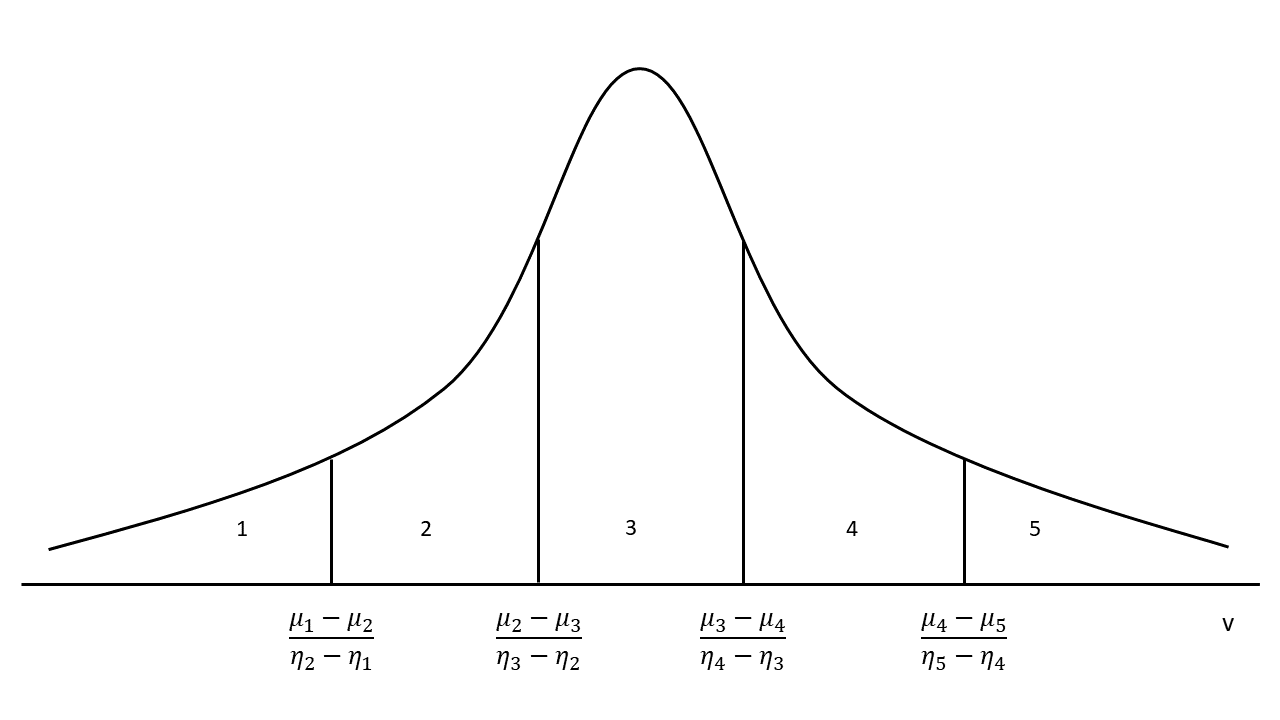
\includegraphics[width=300pt]{Bell.png}\\
  \caption{Residential location in a 5-region model, without mobility costs.}\label{pic1}
\end{figure}

\section{Data and identification}\label{fourth_section}

To test the prediction of the theory in China, we analyze the 2010-2016 waves of the China Family Panel Studies (CFPS). The nation-wide CFPS baseline survey in 2010 successfully interviewed 14,798 households, along with 33,600 adults and 8,990 children within these families, in 25 designated provinces, for an approximately response rate of 79\%. The stratified multi-stage sampling 7 strategy ensures that the CFPS sample represents 94.5\% of the total population in China in 2010. Individual-level follow-up surveys for CFPS adults are conducted every two years. In 2016, CFPS successfully followed up 12,130 of the original households.\\

The identification is based on the two predictions of the theory. The theory predicts that correlation between skill levels and out-migration rates should be more positive in provinces with little earnings inequality than in states with a large amount of dispersion. To test this implication, we can estimate probit models in which the dependent variable is a dummy identifying these individuals who left their native provinces, and the independent variables include measures of skills and controls. \\

The theory also predicts that skilled workers move to provinces with greater wage dispersion and unskilled workers move to provinces with less wage dispersion. We begin testing this hypothesis by estimating OLS regression of the change in wage dispersion (between birthplace and current residence) on measures of skills and other controls. An alternative way of testing this prediction is to model the direction but not the magnitude of the change in wage dispersion. Using the probit model, the dependent variable is each migrant's two choices: move to a state with higher wage dispersion or a lower wage dispersion than the native state. The independent variables include measures of skills and controls.\\\\





\bibliographystyle{apacite}
\bibliography{reference}


\end{document}
